\chapter{Конструкторский раздел}

\section{Функциональная модель оптимизации метода сжатия страниц}

Разрабатываемая оптимизация метода сжатия страниц памяти с использованием подсчета информационной энтропии состоит из следующих этапов:

\begin{enumerate}
	\item Вычисление значения информационной энтропии с помощью метода подсчета.
	\item Сравнение вычисленного значения информационной энтропии с пороговым значением.
	\item Сжатие данных страницы в случае, если полученное значение информационной энтропии меньше порогового значения.
\end{enumerate}

IDEF0-диаграмма первого уровня, формализующая основные этапы оптимизации сжатия страниц оперативной памяти, приведена на рисунке \ref{img:first-level}.
    
\includeimage
    {first-level}
    {f}
    {h}
    {1.0\textwidth}
    {IDEF0-диаграмма первого уровня}

\section{Требования к разрабатываемому программному обеспечению}

Согласно описанию этапов решения поставленной задачи разрабатываемое программное обеспечение должно:

\begin{itemize}
	\item вычислять информационную энтропию страницы оперативной памяти, которая является вектором $a = (a_1\text{ }a_2\text{ }\dotso\text{ }a_N)$ размером $N$, равным размеру страницы памяти, $0 \leq a_i \leq 255$;
	\item если вычисленное значение меньше порогового, сжимать данные входной страницы память, то есть, получать вектор $b = (b_1\text{ }b_2\text{ }\dotso\text{ }b_N)$ размером $N$, $0 \leq b_i \leq 255$;
	\item если вычисленное значение больше или равно пороговому, данные входной страницы памяти не должны изменяться.
\end{itemize}

\section{Структура разрабатываемого программного обеспечения}

Структура загружаемого модуля ядра zram включает в себя следующие части:
\begin{itemize}
	\item модуль блочного устройства, который выполняет функции создания, настройки и удаления дисков, обработки операций записи и чтения страниц и получения статистики;
	\item модуль сжатия, который выполняет функции сжатия и восстановления данных, а также настройку этих операций.
\end{itemize}

Функция сжатия данных, предоставляемая модулем сжатия, вызывается в модуле блочного устройства во время обработки записи страницы на диск, как представлено на рисунке \ref{img:zram-structure}.

\includeimage
    {zram-structure}
    {f}
    {h}
    {0.6\textwidth}
    {Структура модуля zram}

Одним из выделенных к разрабатываемому программному обеспечению требованием является то, что сжатие страницы должно проводиться только в случае, если полученное значение информационной энтропии меньше порогового. Поэтому для выполнения поставленной задачи необходимо изменить функцию записи страницы на диск модуля блочного устройства. Структура разрабатываемого программного обеспечения показана на рисунке \ref{img:structure}.

\begin{figure}[H]
	\begin{center}
		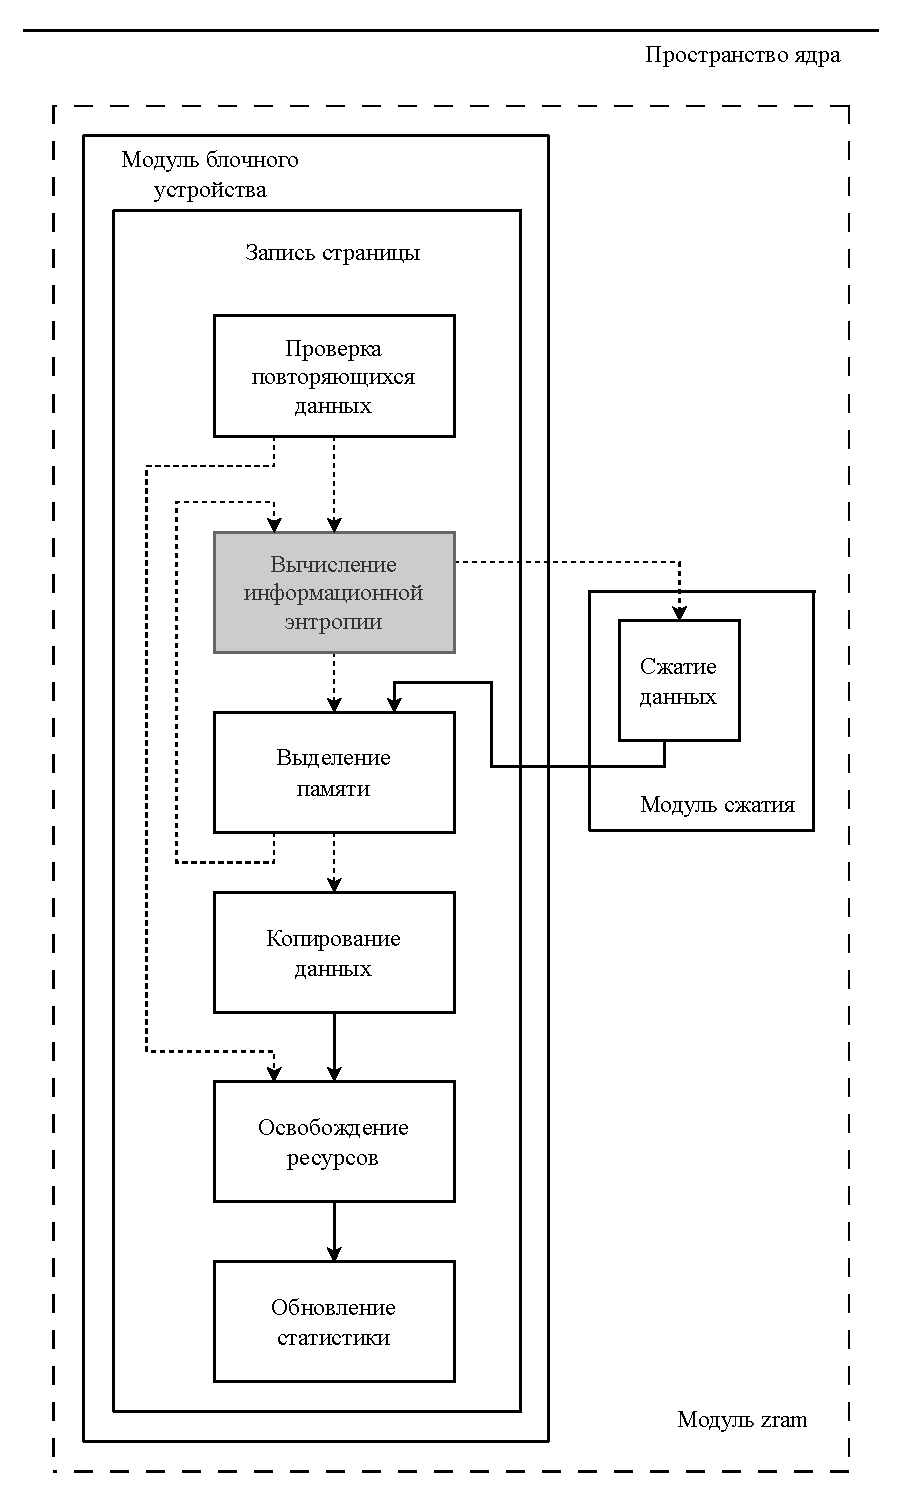
\includegraphics[scale=0.6]{inc/img/structure.pdf}
	\end{center}
	\captionsetup{justification=centering}
	\caption{Структура разрабатываемого программного обеспечения}
	\label{img:structure}
\end{figure}

\section{Схемы алгоритмов}

На основе описания метода скользящего окна для подсчета информационной энтропии из раздела \ref{sliding-window} была построена схема данного алгоритма, приведенная на рисунке \ref{img:get-sw-entropy}.

\begin{figure}[H]
	\begin{center}
		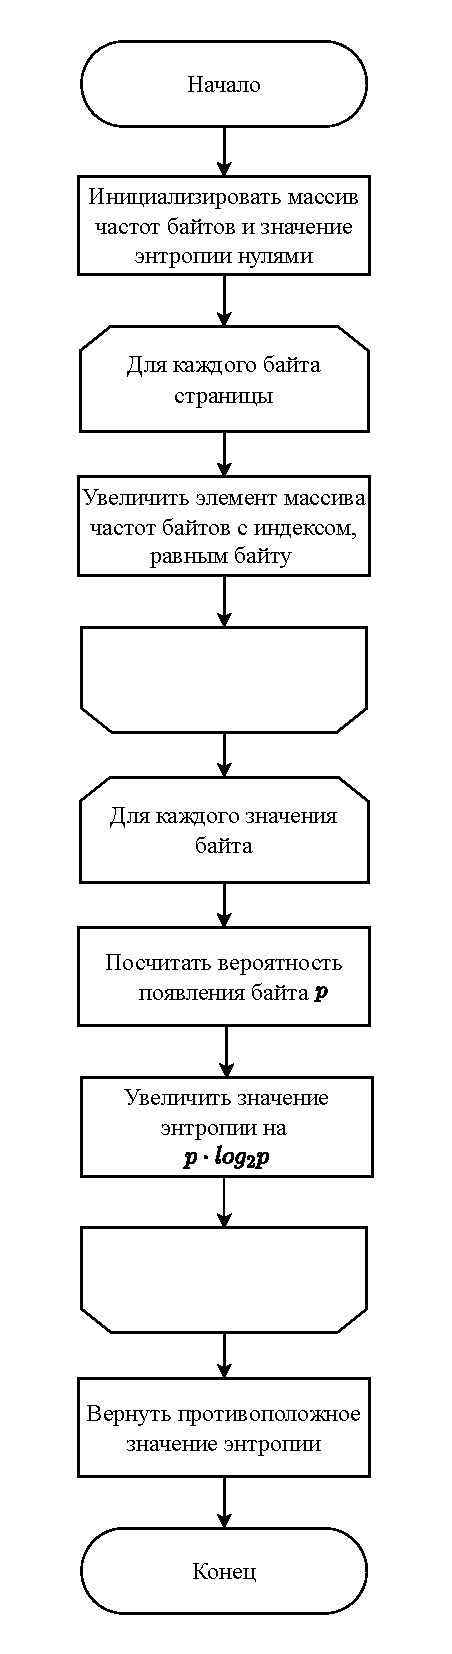
\includegraphics[scale=0.7]{inc/img/get-sw-entropy.pdf}
	\end{center}
	\captionsetup{justification=centering}
	\caption{Схема алгоритма метода скользящего окна}
	\label{img:get-sw-entropy}
\end{figure}

На основе описания биномиального метода подсчета информационной энтропии из раздела \ref{binomial} была построена схема данного алгоритма, приведенная на рисунке \ref{img:get-binomial-entropy}.

\begin{figure}[H]
	\begin{center}
		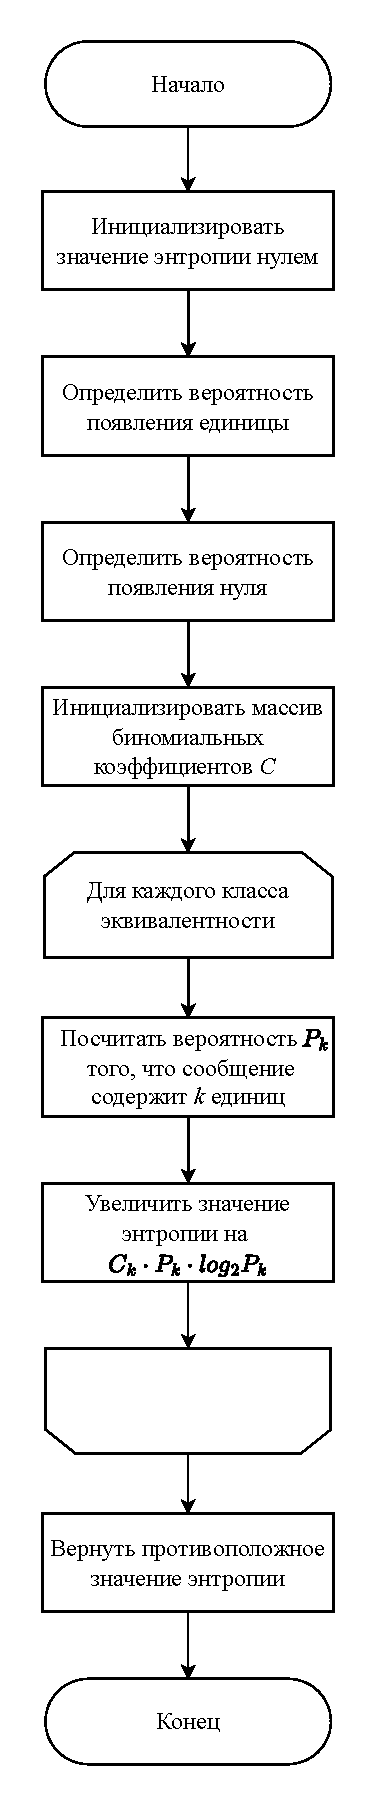
\includegraphics[scale=0.7]{inc/img/get-binomial-entropy.pdf}
	\end{center}
	\captionsetup{justification=centering}
	\caption{Схема алгоритма биномиального метода}
	\label{img:get-binomial-entropy}
\end{figure}

В результате анализа исходного кода загружаемого модуля zram \cite{zram-code} и описания этапов разрабатываемой оптимизации метода сжатия страниц памяти была построена схема алгоритма записи страницы на диск, представленная на рисунке \ref{img:write-page}.

\begin{figure}[H]
	\begin{center}
		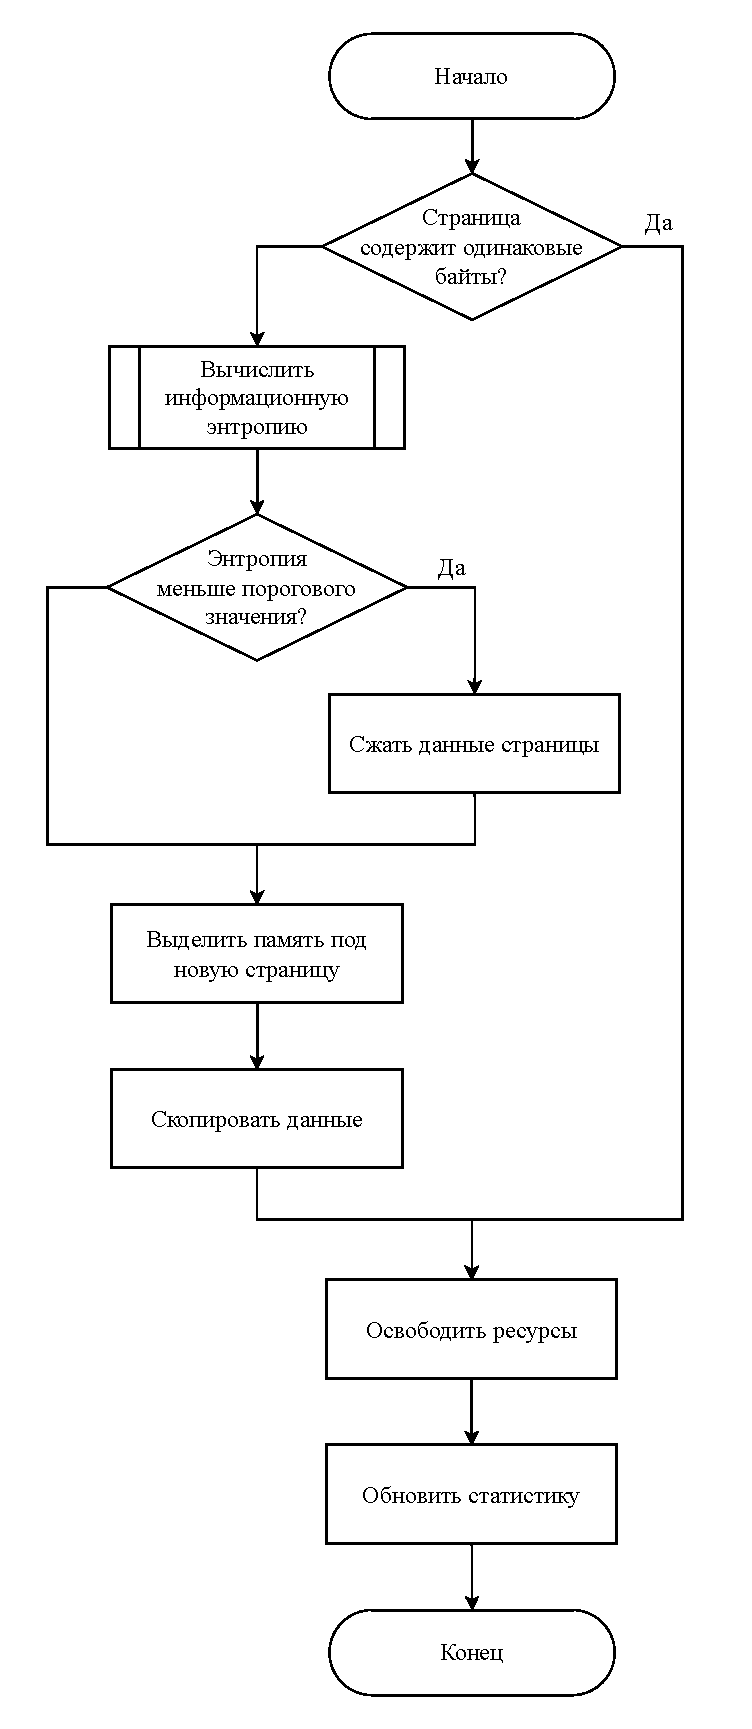
\includegraphics[scale=0.7]{inc/img/write-page.pdf}
	\end{center}
	\captionsetup{justification=centering}
	\caption{Схема алгоритма записи страницы на диск}
	\label{img:write-page}
\end{figure}

\section{Выбор типов и структур данных}

Входными и выходными данными является страница памяти, которая задается вектором размером меньшим или равным размеру страницы в байтах, состоящим из значений от нуля до 255. Поэтому для представления страницы в методе подсчета информационной энтропии должен использоваться массив типа unsigned char размером, равным размеру страницы в байтах.

При выполнении операций с числами с плавающей точкой в режиме пользователя ядро перехватывает системное прерывание и переходит из режима вычислений с целыми числами в режим с плавающей точкой. Если использовать режим с плавающей точке в пространстве ядра, необходимо сохранять и восстанавливать состояние регистров с плавающей точкой математического сопроцессора. Вычисления с числами с плавающей точкой в режиме ядра выполнять не рекомендуется. Поэтому для представления числовых величин должен использоваться целочисленный тип данных. 

\section{Тестирование разрабатываемого программного обеспечения}

Проверка и отладка разрабатываемого программного обеспечения должны проводиться с помощью ручного тестирования.

Система для выполнения тестирования включает следующие компоненты:

\begin{itemize}
	\item персональный компьютер, который является хостом;
	\item виртуальная машина, на которой загружен модуль zram без разрабатываемой оптимизации;
	\item виртуальная машина, на которой загружен модуль zram с разрабатываемой оптимизацией.
\end{itemize}

Схема тестирующей системы показана на рисунке \ref{img:testing-scheme}.

\includeimage
    {testing-scheme}
    {f}
    {h}
    {0.5\textwidth}
    {Схема системы для тестирования}

Для проведения тестирования выделены следующие классы эквивалентности:

\begin{enumerate}
	\item Несжимаемые страницы памяти;
	\item Сжимаемые страницы памяти.
\end{enumerate}

Несжимаемыми страницами памяти являются страницы с высоким значением энтропии. В разделе \ref{relation} было доказано, что энтропия сжатых данных выше энтропии исходных данных. Поэтому тестовый набор для первого класса эквивалентности должен включать сжатые данные. Примерами таких данных являются файлы форматов zip, png, mp3.

Сжимаемыми страницами памяти являются страницы данных с выделяемой структурой, как было сказано в разделе \ref{relation}. Примерами таких данных являются файлы форматов txt и doc, из которых должен состоять тестовый набор для второго класса эквивалентности.

\section*{Вывод}

В данном разделе были разработаны основные этапы оптимизации метода сжатия страниц памяти с использованием подсчета информационной энтропии. Были сформулированы требования к разрабатываемому программному решению. Взаимодействие компонентов системы было представлено в виде структуры. Кроме того были представлены схемы алгоритмов подсчета информационной энтропии и записи страниц на диск модулем блочного устройства загружаемого модуля zram. Был обоснован выбор целочисленного типа данных и массива в качестве структуры, представляющей страницу памяти.
